\documentclass[12pt]{article}
 
\usepackage[margin=1in]{geometry} 
\usepackage{amsmath,amsthm,amssymb}

\usepackage[brazilian]{babel}
\usepackage[utf8]{inputenc}
\usepackage[T1]{fontenc}
\usepackage{graphicx}         %pacote para incluir figuras tipo eps
\usepackage{xcolor}
\usepackage{float} 
\usepackage{epstopdf}
 
 %Matlab code in latex 
\usepackage[final]{listings}
\usepackage{color} %red, green, blue, yellow, cyan, magenta, black, white
\definecolor{mygreen}{RGB}{28,172,0}
\definecolor{mylilas}{RGB}{170,55,241}
\lstdefinestyle{myMatlab}
{
language=matlab,frame=single, basicstyle=\small\ttfamily,breaklines=true,%
morekeywords={matlab2tikz}, keywordstyle=\color{blue}, morekeywords=[2]{1}, keywordstyle=[2]{\color{black}}, commentstyle=\color{mygreen}, stringstyle=\color{mylilas}, identifierstyle=\color{black}, showstringspaces=false,%without this there will be a symbol in the places where there is a space
numbers=left, numberstyle={\scriptsize \color{black}},% size of the numbers
numbersep=9pt, % this defines how far the numbers are from the text
% emph=[1]{for,end,break},emphstyle=[1]\color{red}, %some words to emphasise
% emph=[2]{word1,word2}, emphstyle=[2]{style},
}
 
\newcommand{\N}{\mathbb{N}}
\newcommand{\Z}{\mathbb{Z}}
 
\newenvironment{theorem}[2][Theorem]{\begin{trivlist}
\item[\hskip \labelsep {\bfseries #1}\hskip \labelsep {\bfseries #2.}]}{\end{trivlist}}
\newenvironment{lemma}[2][Lemma]{\begin{trivlist}
\item[\hskip \labelsep {\bfseries #1}\hskip \labelsep {\bfseries #2.}]}{\end{trivlist}}
\newenvironment{exercise}[2][Exercício]{\begin{trivlist}
\item[\hskip \labelsep {\bfseries #1}\hskip \labelsep {\bfseries #2.}]}{\end{trivlist}}
\newenvironment{reflection}[2][Reflection]{\begin{trivlist}
\item[\hskip \labelsep {\bfseries #1}\hskip \labelsep {\bfseries #2.}]}{\end{trivlist}}
\newenvironment{proposition}[2][Proposition]{\begin{trivlist}
\item[\hskip \labelsep {\bfseries #1}\hskip \labelsep {\bfseries #2.}]}{\end{trivlist}}
\newenvironment{corollary}[2][Corollary]{\begin{trivlist}
\item[\hskip \labelsep {\bfseries #1}\hskip \labelsep {\bfseries #2.}]}{\end{trivlist}}
 
\begin{document}
 
% --------------------------------------------------------------
%                         Start here
% --------------------------------------------------------------
 
\title{Exercício 01}
\author{Renan Salles de Freitas\\
CPE 723 - Otimização Natural}
 
\maketitle
 
\begin{exercise}{1.a} 
\begin{align*}
\int xe^{-x} dx = \int -x d(e^{-x}) &= -xe^{-x} + \int e^{-x} dx \\
\int xe^{-x} dx = -xe^{-x} - e^{-x} &= -e^{-x} (x+1)  \\
\int_{0}^{1} xe^{-x} dx = \frac{e-2}{e} &= \approx 0.26424
\end{align*}
\end{exercise}
 
\begin{exercise}{1.b}\\
Segue o código fonte do exercício, em Matlab:
\lstinputlisting[style=myMatlab]{matlab/exercicio0101b.m} 
\end{exercise}

\begin{exercise}{1.c}
Queremos encontrar $I = \int_{0}^{1} xe^{-x} dx$. Podemos reescrever a integral
como valor esperado $I = \mathbb{E}[f(X)]$, onde $f$ é alguma função real e $X$
é uma variável aleatória cuja distribuição de probabilidade é definida por
alguma função de densidade de probabilidade.

Temos que $X \thicksim \phi(x) = \lambda e^{-\lambda x} $. Devemos
normalizar a função de densidade de probabilidade para o intervalo $(0,1)$,
logo:
\begin{align*}
\phi(x) &=  \frac{\lambda e^{-\lambda x}}{\int_0^1 \lambda e^{-\lambda x} dx} \\
\phi(x) &=  \frac{\lambda e^{-\lambda x}}{1-e^{-\lambda}}
\end{align*}

Temos ainda que:
\begin{align*}
\mathbb{E}[f(X)] &= \int_0^1 f(t)\phi(t) dt \\
\mathbb{E}[f(X)] &= \int_0^1 f(t)\frac{\lambda e^{-\lambda x}}{1-e^{-\lambda}} dt
\end{align*}

Para chegarmos em $I$, escolhemos $\lambda = 1$ e $f(x)$:
\begin{align*}
f(t) &= (1-e^{-1})t
\end{align*} 
  
E assim temos:
\begin{align*}
I = \int_{0}^{1} te^{-t} dt
\end{align*}

A integração pelo método de Monte Carlo diz que se $X_1, \ldots, X_N$ são
amostras independentes da distribuição exponencial $X \thicksim \phi(x) = e^{-x}
$, então:

\begin{align*}
\lim_{N\rightarrow +\infty} \frac{1}{N} \sum_{i=1}^{N} f(X_i) &=
\mathbb{E}[f(X)] \\
I &= \sum_{i=1}^{N} X_i
\end{align*}

Utilizando o programa escrito em MatLab, abaixo:
\lstinputlisting[style=myMatlab]{matlab/exercicio0101c.m}

Obtivemos $I = 0.2687$ para $10$ amostras. 

\end{exercise}

\begin{exercise}{2}
Considere:
\begin{align*}
f(x,y) &= \begin{cases}
1 & x^2 + y^2 \leq 1\\
0 & x^2 + y^2 \geq 1
\end{cases}
\end{align*}
E considere o domínio $D = [-1,1] \times [-1,1]$. Temos que:
\begin{align*}
\int_D f(x,y)dxdy = \pi
\end{align*}
Podemos estimar o valor de $\pi$ pelo método de integração de Monte Carlo,
escolhendo N números de maneira aleatória em $D$:
\begin{align*}
\pi \approx \frac{4}{N}\sum_{i=1}^{N}f(x_i,y_i)
\end{align*}

Usando $N=20$, obtivemos como resultado $\pi = 2.8$. Usando $N=1.000.000$,
obtivemos $\pi = 3.1411$. O resultado se aproxima cada vez mais de $\pi$ quanto
maior for o valor de $N$. Esse resultado é provado pela lei dos grandes números:
quanto mais tentativas são realizadas, mais a probabilidade da média aritmética
dos resultados observados irá se aproximar da probabilidade real.

\lstinputlisting[style=myMatlab]{matlab/exercicio02.m} 
\end{exercise}

\begin{exercise}{3.a}

Segue o código fonte do exercício, em Matlab:

\lstinputlisting[style=myMatlab]{matlab/exercicio03.m}

\begin{figure}[H]
  \centering
  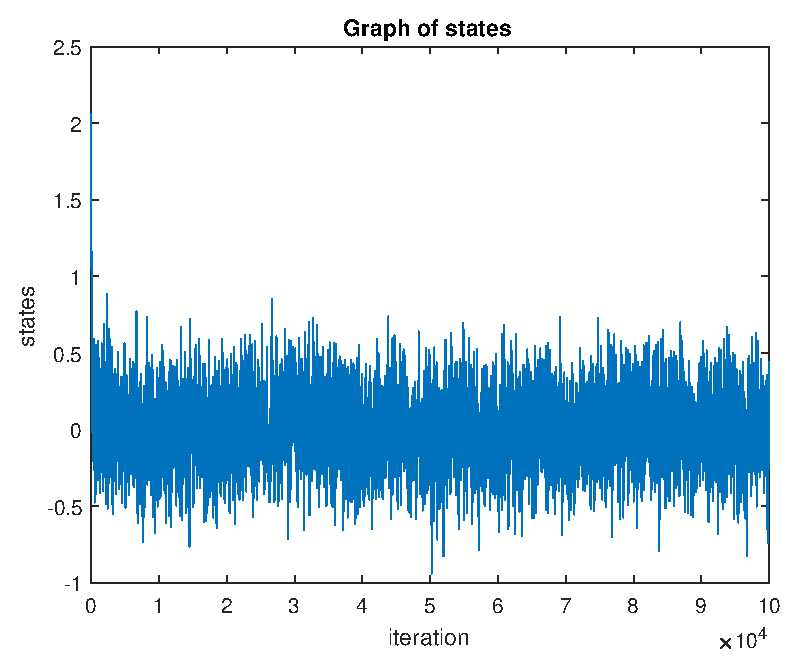
\includegraphics[width=12cm]{figs/ex3_states.eps} 
\end{figure}

\begin{figure}[H]
  \centering
  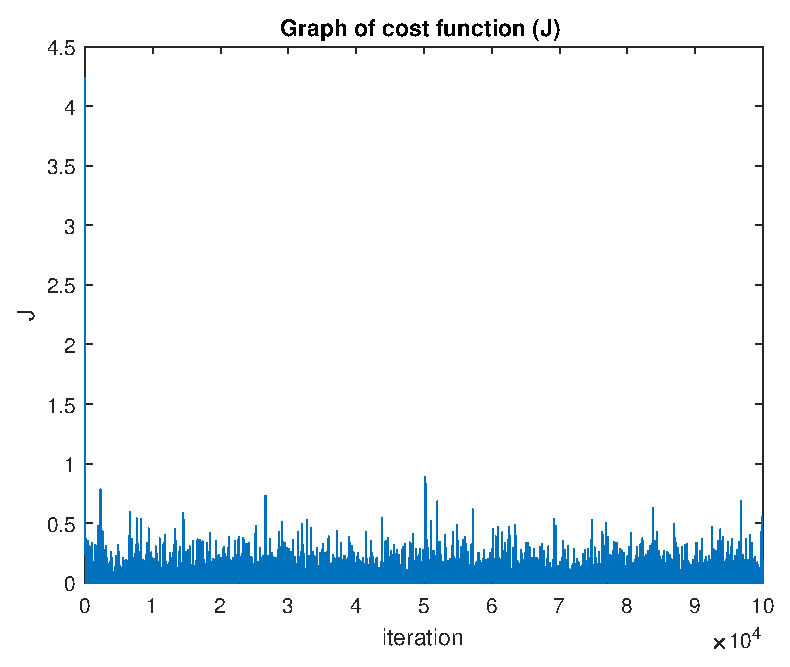
\includegraphics[width=8cm]{figs/ex3_j.eps} 
\end{figure}
\end{exercise}

\begin{exercise}{3.b}
Resolução de dez iterações do algoritmo:
\begin{align}
x_0 &= 2 \\
\nonumber r &= -0.9091 \\
\nonumber x_1 &= x_0 + 0.1*(-0.9091) = 1.9091 \\
\nonumber \Delta J &= x_1^2 - x_0^2 = -0.3554 < 0 \\ 
\nonumber x_1 &= 1.9091
\end{align}

\begin{align}
x_1 &= 1.9091 \\
\nonumber r &= -0.3739 \\
\nonumber x_2 &= x_1 + 0.1*(-0.9975) = 1.8717 \\
\nonumber \Delta J &= x_2^2 - x_1^2 = -0.1414 < 0 \\ 
\nonumber x_2 &= 1.8717
\end{align}

\begin{table}[H]
\centering
\label{t01}
\begin{tabular}{ccccccc}
$X_k$  & r       & \multicolumn{1}{l}{$\hat{X}$} & $\Delta J$ & $e^{-\frac{\Delta J}{T}}$ & a      & $X_{k+1}$ \\
2      & -0.9091 & 1.9091                        & -0.3554    & -                         & -      & 1.9091    \\
1.9091 & -0.3739 & 1.8717                        & -0.1414    & -                         & -      & 1.8717    \\
1.8717 & 0.8264  & 1.9543                        & 0.3162     & 0.0424                    & 0.5054 & 1.8717    \\
1.8717 & 0.8098  & 1.9527                        & 0.3097     & 0.0452                    & 0.1342 & 1.8717    \\
1.8717 & -0.3808 & 1.8336                        & -0.1411    & -                         & -      & 1.8336    \\
1.8336 & -0.4297 & 1.7906                        & -0.1557    & -                         & -      & 1.7906    \\
1.7906 & 0.2195  & 1.8126                        & 0.0791     & 0.4535                    & 0.4008 & 1.8126    \\
1.8126 & 0.2301  & 1.8356                        & 0.0839     & 0.4320                    & 0.9469 & 1.8126    \\
1.8126 & 0.6654  & 1.8791                        & 0.2456     & 0.0857                    & 0.4103 & 1.8126    \\
1.8126 & 0.0788  & 1.8205                        & 0.0286     & 0.7509                    & 0.0656 & 1.8205   
\end{tabular}
\end{table}

\end{exercise}

\begin{exercise}{4}

A função custo (J) pode ser vista na figura~\ref{fig:j04}. Segue o código fonte
do exercício, em Matlab:

\lstinputlisting[style=myMatlab]{matlab/exercicio04b.m}

\begin{figure}[H] 
  \centering
  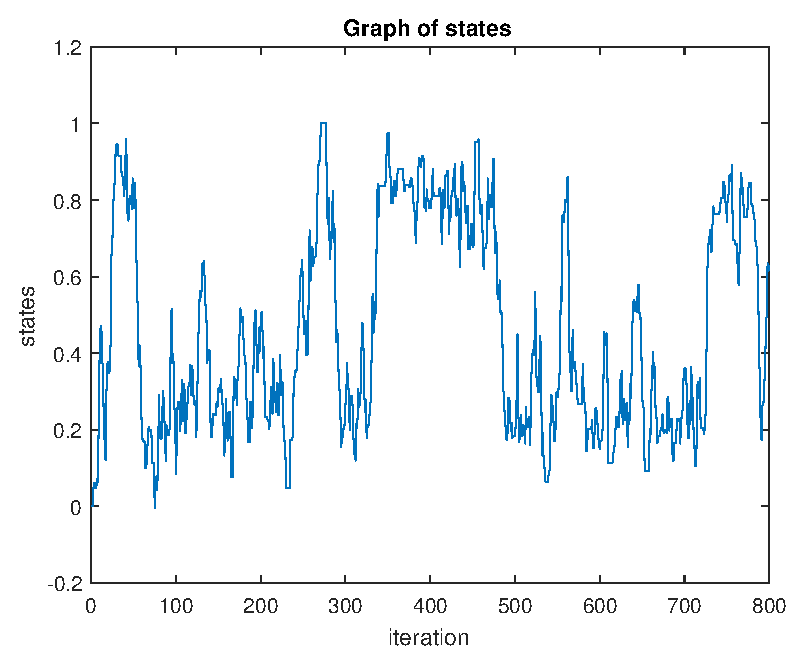
\includegraphics[width=12cm]{figs/ex4b_states.eps} 
\end{figure}

\begin{figure}[H]
  \centering
  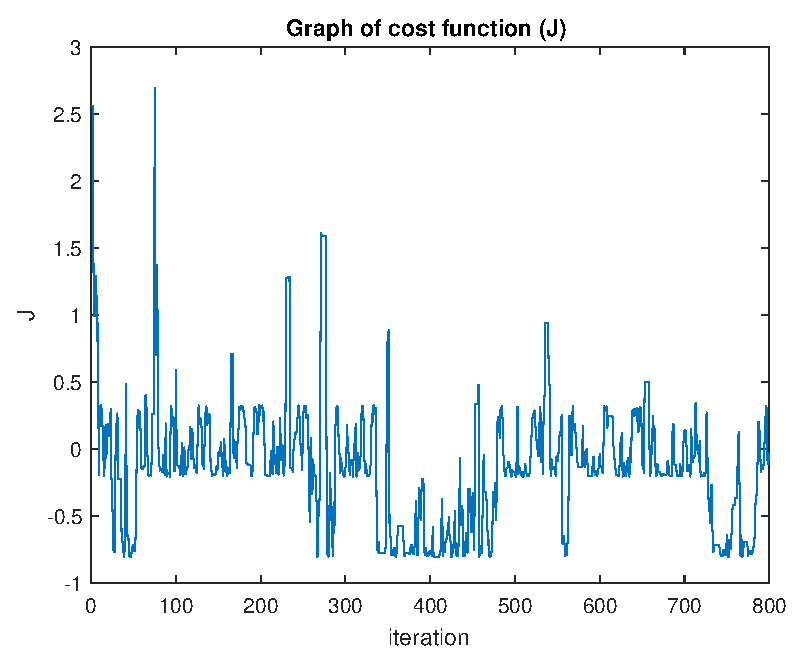
\includegraphics[width=12cm]{figs/ex4b_j.eps} 
\end{figure}

\begin{figure}[H]
  \centering
  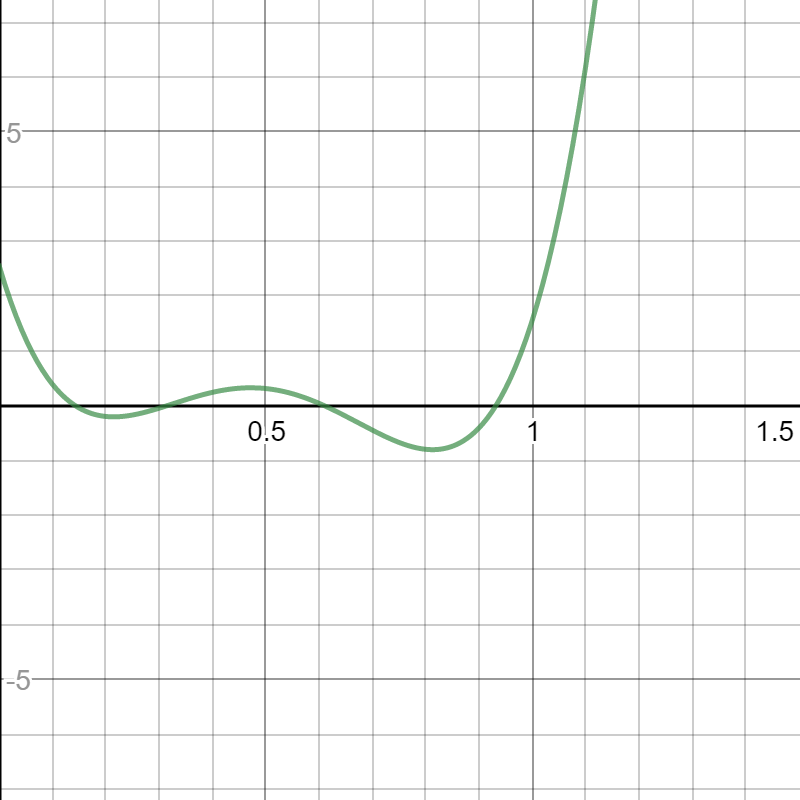
\includegraphics[width=12cm]{figs/j_04.png}
  \caption{Gráfico da função J}
  \label{fig:j04} 
\end{figure}
 
Obtivemos $x_{\text{min}} = 0.8135$ e $J(x_{\text{min}}) = -0.8066$.
 
Calculando as primeiras iterações para $T = 1$ e $x_0 = 0$
\begin{table}[H]
\centering
\begin{tabular}{ccccccc}
$X_k$  & r       & \multicolumn{1}{l}{$\hat{X}$} & $\Delta J$ & $e^{-\frac{\Delta J}{T}}$ & a      & $X_{k+1}$ \\
0      & -0.6576 & -0.0658                       & 2.7998     & 0.0608                    & 0.1627 & 0         \\
0      & -0.7593 & -0.0759                       & 3.3574     & 0.0348                    & 0.6375 & 0         \\
0      & 0.8124  & 0.0812                        & -1.9126    & -                         & -      & 0.0812    \\
0.0812 & 0.0695  & 0.0882                        & -0.1023    & -                         & -      & 0.0882    \\
0.0882 & -1.8337 & -0.0952                       & 6.5316     & 0.0015                    & 0.8828 & 0.0882    \\
0.0882 & 1.8274  & 0.2709                        & -0.6752    & -                         & -      & 0.2709    \\
0.2709 & 0.6541  & 0.3363                        & 0.1934     & 0.8242                    & 0.2174 & 0.3363    \\
0.3363 & -1.5448 & 0.1818                        & -0.2324    & -                         & -      & 0.1818    \\
0.1818 & -0.3751 & 0.1443                        & 0.1583     & 0.8536                    & 0.7199 & 0.1443    \\
0.1443 & 0.2077  & 0.1651                        & -0.1050    & -                         & -      & 0.1651   
\end{tabular}
\end{table}
Vale observar como o algoritmo oscila no mínimo local, mas pode alcançar o
mínimo global, como na iteração 8. 
\end{exercise}

\begin{exercise}{5}
A função que queremos minimizar é a Rosenbrock function, descrita com:
\begin{align*}
f(x,y) &= (1-x)^2 + 100(y-x^2)^2
\end{align*}
O mínimo da função se encontra em $(x,y) = (1,1)$ e $f(x,y) = 0$. Modificamos o
algoritmo SA para vetores de duas dimensões, como pode ser visto abaixo:

\lstinputlisting[style=myMatlab]{matlab/exercicio05.m}

\begin{figure}[H]
  \centering
  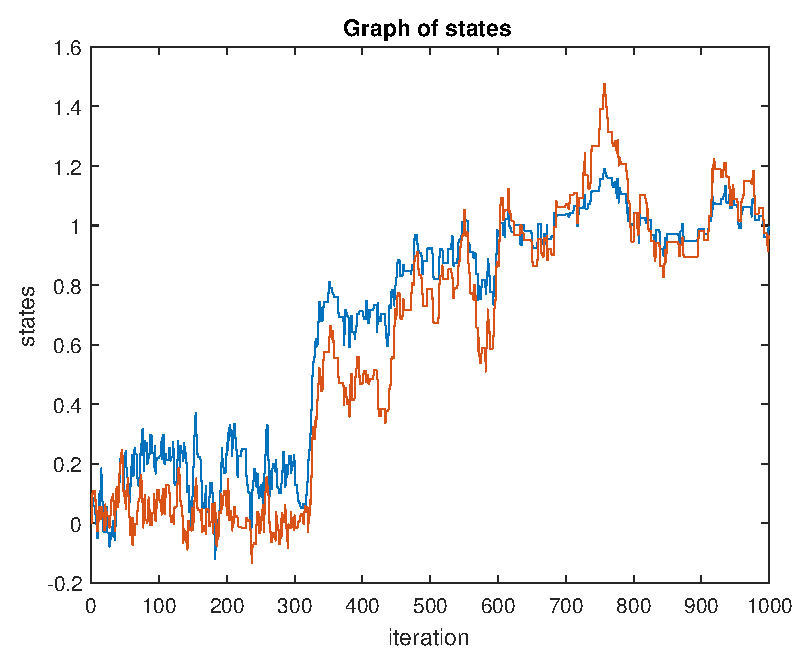
\includegraphics[width=12cm]{figs/ex5_states.eps} 
\end{figure}

\begin{figure}[H]
  \centering
  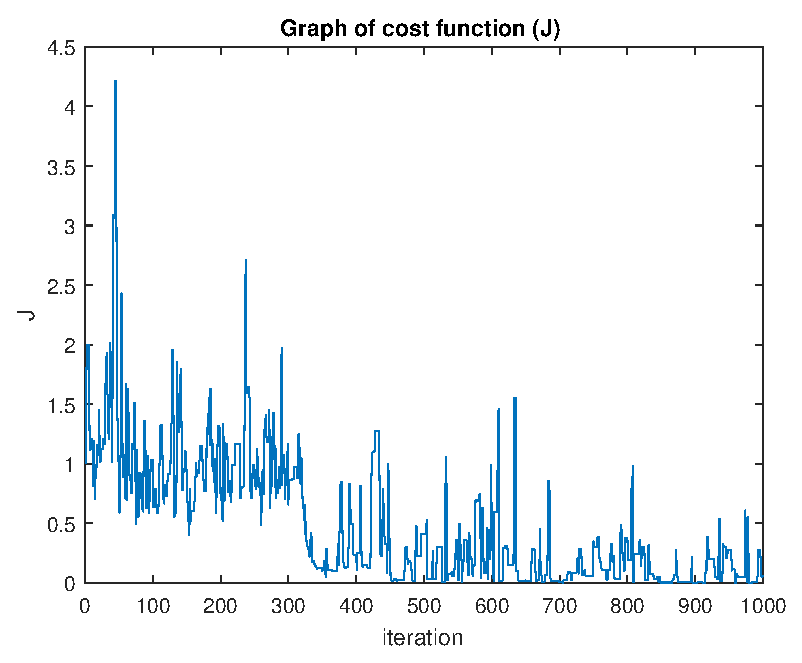
\includegraphics[width=12cm]{figs/ex5_j.eps} 
\end{figure}

Obtivemos $x_{\text{min}} = (1.0168, 1.0311)$ e $J(x_{\text{min}}) = 0.001$.

\end{exercise}
 
\end{document}
              
